
\section{Background and API}
Now, we will overview some of the preliminary concepts and describe how this formalism inspires a modular system API.

\subsection{Basic Setup}
\vspace{0.25em} \noindent \textbf{Language: } Let $R$ be a relation over a set of attributes $A$, and let $\mathcal{R}$ denote the set of all possible relations over $A$.
A data transformation is an operator over $\mathcal{R}$: 
\[T(R): \mathcal{R} \mapsto  \mathcal{R}\]
Let $\Sigma$ define a set of distinct transformations $\{T_1, T_2,..,T_N\}$.
Let $\Sigma^*$ be the set of all finite subsequences of $\Sigma$, i.e., $T_i(T_j(R))$.
A formal language $L$ over  $\Sigma$ is a subset of $\Sigma^*$.

\vspace{0.5em} \noindent \emph{Example 1: } As an example, given below is a relation with two attributes \textsf{city\_name} and \textsf{city\_code}. 
Assuming unique city names, there should be a one-to-one map between city names and the city code. The problem is that the relation we have is inconsistent.

\begin{table}[ht!]
\centering
\label{my-label}
\begin{tabular}{|l|l|l|}
\hline
\rowcolor[HTML]{000000} 
& {\color[HTML]{FFFFFF} city\_name}            & {\color[HTML]{FFFFFF} city\_code}   \\ \hline
1 & San Francisco                                & SF                                  \\ \hline
2& {\color[HTML]{FE0000} \textbf{New York}}     & NY                                  \\ \hline
3 & New York City                                & {\color[HTML]{FE0000} \textbf{NYC}} \\ \hline
4 & {\color[HTML]{FE0000} \textbf{San Francisc}} & SF                                  \\ \hline
5 & San Jose                                     & SJ                                  \\ \hline
6 & San Mateo                                    & SM                                  \\ \hline
7 & New York City                                & NY                                  \\ \hline
\end{tabular}
\end{table}

Consider the following function:
\[
\textsf{find\_replace}(\text{source}, \text{target}, \text{attribute})
\]
This function finds all cells with the source string, and replaces it with a target string, in the specified attribute.
If we consider exact string matches and only target strings in the attribute's current domain, there are $61$ possible operations for the example relation.
The set of all find-and-replace operations defines $\Sigma$.
$\Sigma^*$ defines any finite sequences composed of these $61$ operations.
$L$ is any subset of $\Sigma^*$. 
For example, we may only want to consider sequences of length $k$.



\vspace{0.5em} \noindent \textbf{Quality Functions: } A quality function $Q$ maps a relation $R$ to a scalar where 1 implies it is clean:
\[
Q: \mathcal{R} \mapsto [0,1]
\]
A separable quality function is one that can be expressed as an average over cell-wise quality metrics $q(r,a)$ where 1 implies clean:
\[
Q(R) \propto \sum_{r \in R} \sum_{a \in A} q(r,a)
\]



\vspace{0.5em} \noindent \emph{Example 2: } One can model this constraint with two functional dependencies: $\textsf{city\_name} \rightarrow \textsf{city\_code}$ and $\textsf{city\_code} \rightarrow \textsf{city\_name}$.
With these functional dependencies, identifying inconsistencies is efficient -- it requires querying for the set cities that map to more than one city code, and vice versa. 
$Q(R)$ is a separable quality metric where each cell is assigned a 0  if it contains a violating key. 


\vspace{0.5em} \noindent \textbf{Optimization Problem: } Given a quality function $Q$, a relation $R$, and a language $L$, find a sequence of transformations $l \in L$ that optimizes the quality function.
\[
\textsf{search}(Q,R,L) = ~ \min_{l \in L} Q( l(R) )  
\]

\vspace{0.5em} \noindent \emph{Example 3: } Let $L$ be the set of all sequences of length $3$ over $\Sigma$ defined in Example 1, R be the data in Example 1, and $Q$ be the quality function described in Example 2.
One solution to the search problem is:
\begin{lstlisting}
find_replace(New York, New York City, city_name)
find_replace(San Francisc, San Francisco, city_name)
find_replace(NYC, NY, city_code)
\end{lstlisting}


\vspace{0.25em} \noindent\textbf{Complexity: } The search problem is extremely general, and it is not our intention to directly solve this problem in full generality.
In fact, we can show that it is APX-Hard--that is, unless P=NP there does not exist a polynomial time approximation scheme.
However, we find that this optimization problem is a good starting point and an analysis of the complexity illustrates a number of important structural features of the problem.

\begin{proposition}
\textsf{search(Q,R,L)} is \textsf{APX-Hard}
\end{proposition}
\begin{proof}[Sketch]
Let $R$ be a single-attribute relation of Booleans. Let $L$ be the set of all assignments to a single value.
Given a list of $N$ Boolean clauses over all the boolean variables, let $Q$ assign to each record one minus the fraction of clauses that evaluate to true. This formulation is equivalent to MAX-SAT and solution to the optimization problem.
\end{proof}

This reduction gives us some insight into what makes this problem computationally hard, and why practical data cleaning problems may not have those features. \emph{(1)} Arbitrary constraint satisfaction problems are challenging because all variables can interact. While this is certainly the case for arbitrary quality functions, in many cases, data errors are localized. For example, replacing \texttt{San Francisc} with \texttt{San Francisco} has no effect on the records referring to \texttt{New York City}.  \emph{(2)} Arbitrary constraint satisfaction involves assignments to all variables. On the other hand, in data cleaning, hopefully the majority of records in a dataset are clean so there is a structure that can be exploited.
 \emph{(3)} Constraint satisfaction does not model context, each variable is simply a Boolean value. In data cleaning, we can pragmatically exploit similarity. Similar records should be cleaned in similar ways.  

Several automatic approaches have been proposed to minimally resolve inconsistent functional dependencies~(see survey ~\cite{DBLP:conf/sigmod/ChuIKW16}), and these algorithms are far more efficient than the proposed search for the proposed example.
With no additional information, the search approach described above would have to evaluate $61^3 = 226981$ transformations, which is clearly impractical even for this small example.
However, this formalism is starting point on which we can add instance-specific optimizations.
In the next section, we describe how instance-specific optimizations can be specified.


\subsection{Search Optimizations}
A formal language framework provides a consistent interface for specifying optimizations. We consider the following types of optimizations:

\vspace{0.5em}\noindent\textbf{Static Optimizations: } A static optimization is a regular expression that all transformation sequences must satisfy independent of the data. 
\[\textsf{static\_opt}(L, \text{regex} ) \mapsto L'\]
For example, since the find-and-replace operations are idempotent, i.e., $T(T(R)) = T(R)$, we may want to only consider the set of all sequences with no neighboring repeated transformations. Similarly, we may also want to prune all search branches that make no effect (i.e., find-and-replace New York with New York).
These two regular expressions alone reduce the overall number of evaluations by $48\%$ in the above example (120050 v.s. 226981 evaluations).
There are several other possible optimizations  such as avoiding changes that reverse previous changes $T_i(T_j(R)) = R$.


\vspace{0.5em}\noindent\textbf{Dynamic Optimizations: } A dynamic optimization can query the data and cost function to generate rules that are instance-specific:
\[\textsf{dyn\_opt}(Q, R, L) \mapsto \text{regex}\]
For example, we may want to ensure that all the evaluations are ``correlated'' with the cost function--that is it makes modifications that are likely to affect the costs.
This is possible if the cost separable where we have a score for each cell. In this case, we can find all the cells in violation of the functional dependencies and make sure that the ``source'' field of the find-and-replace operations only match values that are in violation.
These optimizations are called ``dynamic' because they can be determined from the active domain (i.e., after applying a transformation, recalculate new optimization rules).
Applying this optimization (in addition to the others) to the example reduces the search space to 1582 evaluations v.s. 226981 unoptimized (143x reduction).

\vspace{0.5em}\noindent\textbf{Blocking Rules: }  Arbitrary constraint satisfaction problems are challenging because all variables can interact. While this is certainly the case for arbitrary quality functions, in many cases, data errors are localized. For example, replacing \texttt{San Francisc} with \texttt{San Francisco} has no effect on the records referring to \texttt{New York City}. The final class of optimizations are blocking rules which have been widely used in entity resolution systems:
\[\textsf{block}(Q, R, L) \mapsto \{R_1,...,R_k\} \]
For quality functions generated from dependencies, we can determine blocks analytically--looking at which violating tuples are linked through the constraint.
However, in general, these blocking rules can be learned (e.g., with clustering) or user defined.
The search can execute on each of the blocks independently.


\vspace{0.5em}\noindent\textbf{Learned Optimizations: } Additionally, \sys can apply machine learning techniques to prune search branches.
To do this, all the transformations in the language have to be featurized to a $d$ dimensional vector:
\[
\textsf{feat}(T) \mapsto \mathbb{R}^d
\]
\sys trains a classifier that maps the d-dimensional vector to $0$ (keep) or $1$ (prune).
This allows the search to execute much faster on future data (or future blocks).

As an example, consider the sequence of transformations described in the example:
\begin{lstlisting}
find_replace(New York, New York City, city_name)
find_replace(San Francisc, San Francisco, city_name)
find_replace(NYC, NY, city_code)
\end{lstlisting}
One observation is that the source and target strings in the optimal sequence are very close in terms of string similarity (as opposed to arbitrary transformations).
If each of these operations was featurized with a single scalar that is the edit-distance between the two strings, then the classifier could learn a pruning threshold (i.e., not considering find-and-replace operations above that threshold).


\subsection{Beyond Classical Data Cleaning}
\sys allows us to go beyond operations typically considered in declarative data cleaning systems and search more complex languages of transformations.

\vspace{0.5em}\noindent\textbf{User-defined transformations: }
One lesson from the above example is that it synthesizes transformations that have no knowledge of the semantics of the data (i.e., we could hash the entire dataset and still get the same results).
The issue with such an approach is that an equally ``optimal'' solution could instead be:
\begin{lstlisting}
find_replace(San Francisco, San Francisc, city_name)
\end{lstlisting}
Problems like this can be avoided with user-defined transformations.
For example, suppose we had a function that given a column deleted all cells that fail a spell check:
\begin{lstlisting}
spellcheck(city_name)
\end{lstlisting}
After applying this transformation, the resulting relation is:
\begin{table}[ht!]
\centering
\label{my-label}
\begin{tabular}{|l|l|l|}
\hline
\rowcolor[HTML]{000000} 
& {\color[HTML]{FFFFFF} city\_name}            & {\color[HTML]{FFFFFF} city\_code}   \\ \hline
1 & San Francisco                                & SF                                  \\ \hline
2& {\color[HTML]{FE0000} \textbf{New York}}     & NY                                  \\ \hline
3 & New York City                                & {\color[HTML]{FE0000} \textbf{NYC}} \\ \hline
4 & {\color[HTML]{005500} \textbf{None}} & SF                                  \\ \hline
5 & San Jose                                     & SJ                                  \\ \hline
6 & San Mateo                                    & SM                                  \\ \hline
7 & New York City                                & NY                                  \\ \hline
\end{tabular}
\end{table}
After this transformation, there is no ambiguity in the minimal repair:
\begin{lstlisting}
spellcheck(city_name)
find_replace(New York, New York City, city_name)
find_replace(None, San Francisco, city_name)
find_replace(NYC, NY, city_code)
\end{lstlisting}
If such a function were available (and we knew when to use it), it would greatly improve the reliability of any subsequent automated cleaning.


\subsection{Program Optimization}
Another benefit to explicitly modeling data cleaning as a program synthesis problem is that the discovered sequence of transformations defines an intermediate
representation, which can be easily transferred between languages or optimized.
For example, consider these operations:
\begin{lstlisting}
find_replace(New York, New York City, city_name)
find_replace(None, San Francisco, city_name)
find_replace(NYC, NY, city_code)
\end{lstlisting}
Since they do not conflict, it would be inefficient to execute them sequentially and iterate over the data three separate times.
Instead, one should combine the operations together and execute at once:
\begin{lstlisting}
for r in rows:
 switch r[city_name]
    case New York: r[city_name] = New York City
    case None: r[city_name] = San Francisco
    default: pass
    
 switch r[city_code]
    case NYC: r[city_code] = NY
    default: pass
\end{lstlisting}


\begin{figure}[t]
% \vspace{-5pt}
\centering
 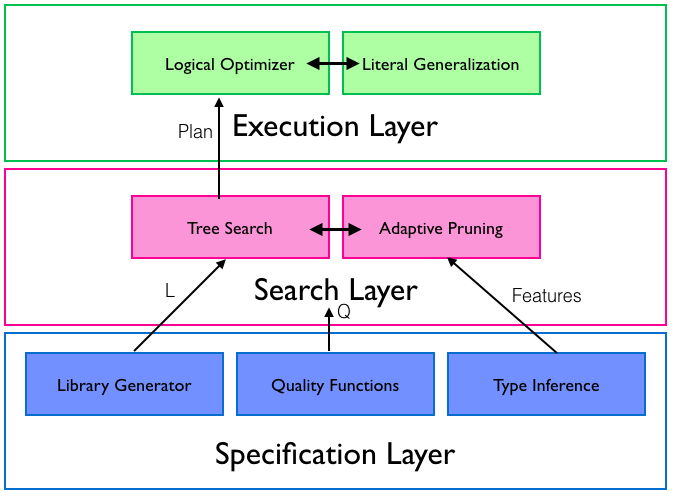
\includegraphics[width=\columnwidth]{figures/alphacleanarch.png}
 \caption{ \sys is given a specification of quality (e.g., integrity constraints or a statistical model the data must conform to) and a language  of  allowed  data  transformations,  and  it  searches  to find a sequence of transformations that maximizes the quality metric. }
\end{figure}








